\chapter{Rekonstruktion}
\label{chap:rekonstruktion}
Zur Verwendung von CDI zur Untersuchung von Proben sind aus dem aufgenommenen Streubild Informationen über die Probe zu rekonstruieren. Wie in \fref{chap:fraunhofer} gezeigt, entspricht die im Fernfeld aufgenommene Welle der Fouriertransformierten der Austrittswelle. Könnte nun sowohl Amplitude als auch Phase des Streubildes aufgenommen werden, so ließe sich durch eine einfache Rücktransformation die Austrittswelle rekonstruieren und somit die gewünschten Informationen über das Objekt gewinnen. Jedoch wird mittels eines Sensors nur die Intensität der Welle aufgezeichnet, die Informationen über die Phase gehen somit verloren. Diese trägt jedoch wie \fref{fig:phaseswap} ersichtlicht einen Großteil der Informationen. Das Problem, aus dieser unvollständigen Messung die Austrittswelle zu rekonstruieren, wird als das Phasenproblem bezeichnet. Zur Lösung existiert seit kurzem der Ansatz der Freiflug-Holographie sowie die etablierte Methode der iterativen Phasenrekonstruktion, die im Folgenden zunächst vorgestellt werden.

\begin{figure}
	\centering
	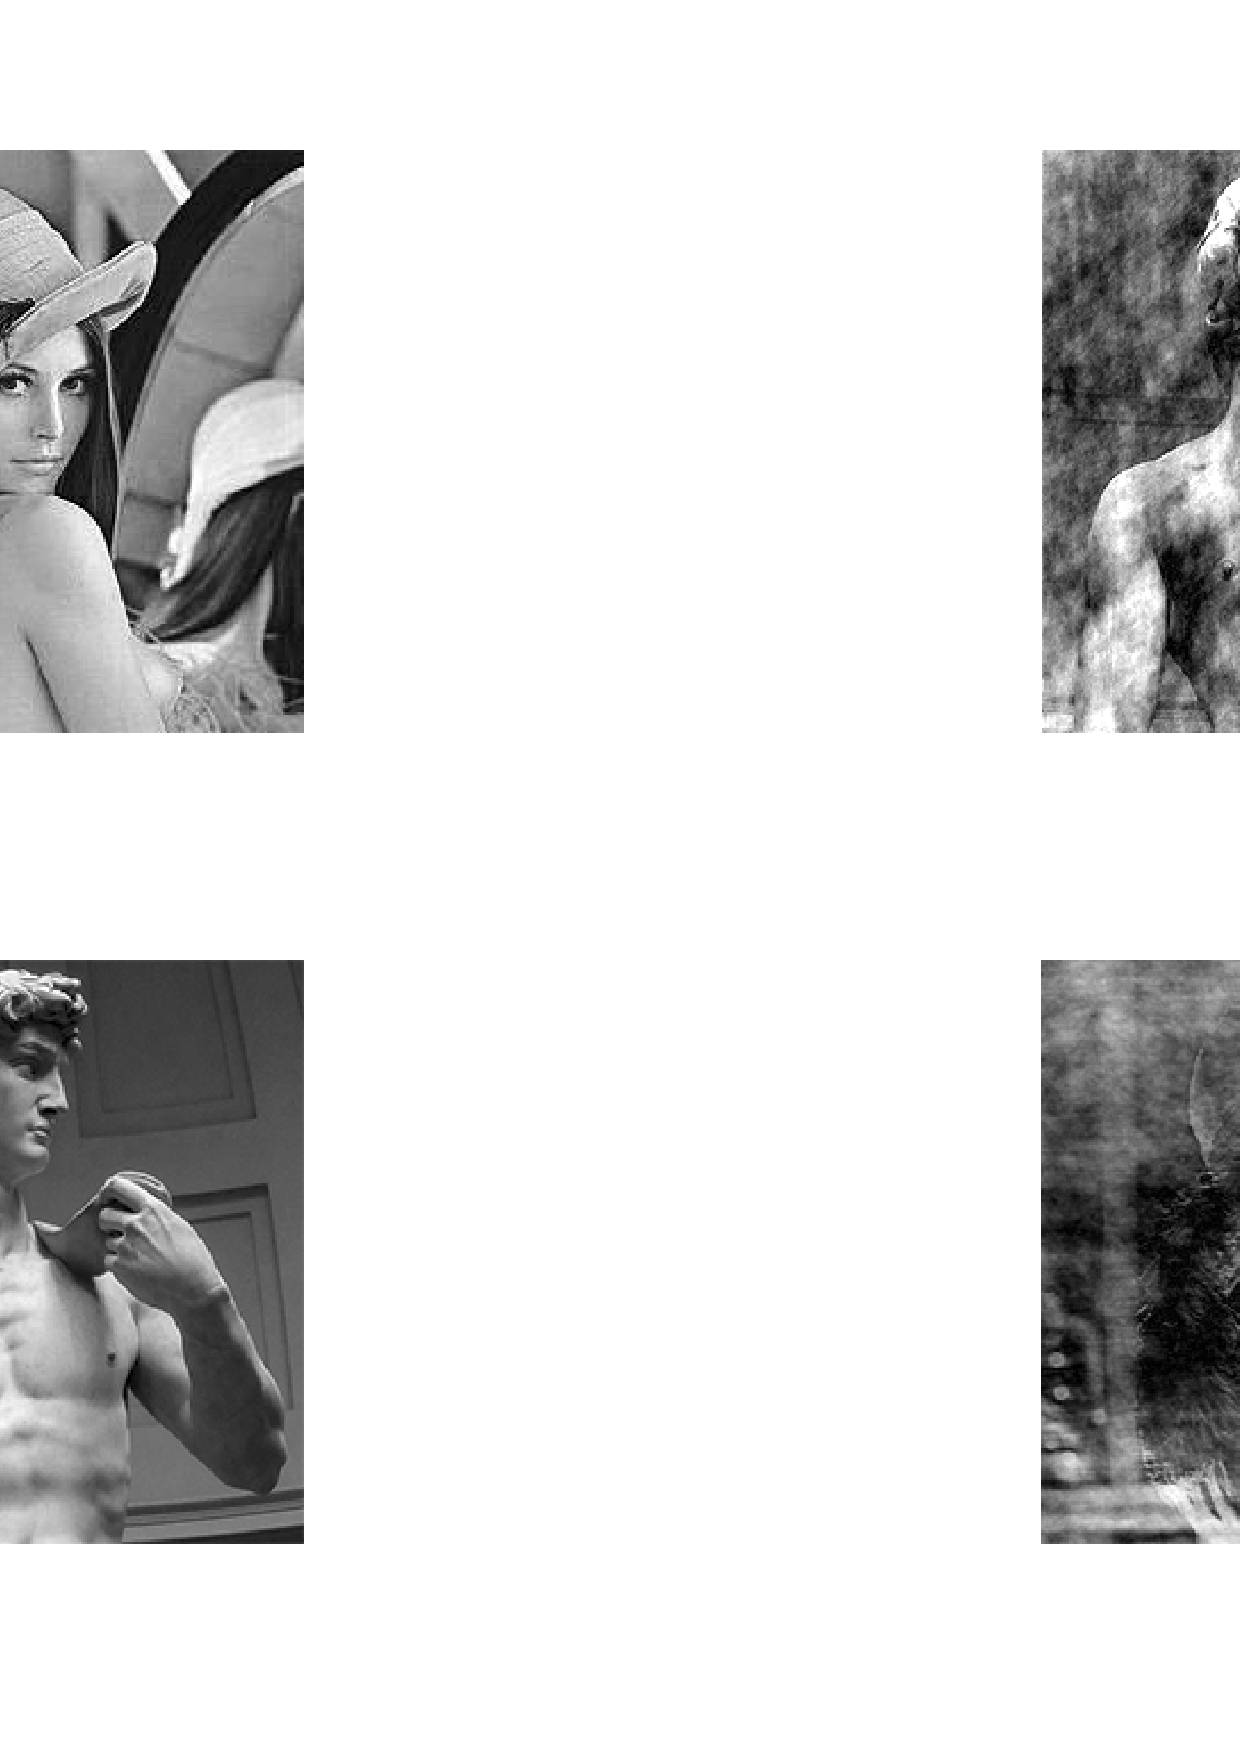
\includegraphics[width=0.75\textwidth]{images/phaseswap.pdf}
	\caption[Bedeutung der Fourierphase]{Zur Illustration der Bedeutung der Fourierphase sind links zwei unterschiedliche Testbilder dargestellt. Aus diesen werden zwei neue Bilder generiert, in dem die Fourieramplituden des einen mit den Phaseninformationen des anderen kombiniert werden. Es ist deutlich zu erkennen, dass hier der visuelle Eindruck von den Phaseninformationen bestimmt wird.}
	\label{fig:phaseswap}
\end{figure}
\section{Holographie}
Bei der Holographie wird versucht, Informationen über die Phase mit aufzuzeichnen. Hierzu wird ein zusätzliches, bekanntes Objekt (im Folgenden als Referenz bezeichnet) in den Strahl eingebracht, sodass die eingehende Welle an beiden gestreut wird. Die Interferenz der beiden gestreuten Wellen kodiert in diesem Fall die relativen Phaseninformationen in der Amplitude.
Das Einbringen einer Referenz wurde in der Vergangenheit üblicherweise realisiert, indem die Probe auf eine Membran mit einer zusätzlichen Öffnung aufgebracht wurde~\cite{eisebitt2004}. Eine elegante Methode, die sog. \textit{Freiflug-Holographie (In-Flight Holography)}, bei der freie Edelgascluster mit in den Strahl eingebracht werden, wurde kürzlich u.a. von Gorkhover und Ulmer vorgestellt~\cite{gorkhover2016,ulmer2015}. 
Sind $O$,$R$ die Austrittswellen von Objekt bzw. Referenz, so gilt für die gemeinsame Austrittswelle $\phi_1$
\begin{equation}
	\phi_1=O+R 
\end{equation}
und für die aufgenommene Intensität $I$ im Fernfeld gilt
\begin{equation}
	I=\left|\mathscr{F}\left[O\right]+\mathscr{F}\left[R\right]\right|^2=\left|\tilde{O}+\tilde{R}\right|^2\,.
\end{equation}
Wird nun auf $I$ eine inverse Fouriertransformation angewendet,

\begin{equation}
	\mathscr{F}^{-1}\left[\left|\tilde{O}+\tilde{R}\right|^2\right]=
	\mathscr{F}^{-1}\left[\tilde{O}\tilde{O}^*\right]+
	\mathscr{F}^{-1}\left[\tilde{R}\tilde{R}^*\right]+
	\mathscr{F}^{-1}\left[\tilde{R}\tilde{O}^*\right]+
	\mathscr{F}^{-1}\left[\tilde{O}\tilde{R}^*\right]\,,
\end{equation}
so ergibt sich mit Hilfe der komplexen Konjugation der Fouriertransformation (\ref{eq:ft_konjugation}) und des Korrelationstheorems (\ref{eq:ft_korrelation})
\begin{equation}
	\mathscr{F}^{-1}[I]\propto \underbrace{O \otimes O + R\otimes R}_{\text{Autokorrelationen}}+\underbrace{R\otimes O+ O\otimes R}_{\text {Kreuzkorrelationen}}\,.
\end{equation}
Dies ist in \fref{fig:fth} illustriert. Die Autokorrelationen, d.h. die Korrelation der Austrittswelle von Objekt mit Objekt bzw. Referenz mit Referenz liegen hierbei um den Ursprung des Koordinatensystems und können in jede Richtung maximal die doppelte Größe von Objekt bzw. Referenz haben. Die Kreuzkorrelationen aus den Austrittswellen von Objekt und Referenz sind punktsymmetrisch zum Ursprung und haben von diesem den gleichen Abstand wie Objekt- und Referenzaustrittswelle voneinander.
Sie  entsprechen einer Faltung des Objektes mit der gespiegelten, komplex konjugierten Referenz bzw. der Referenz mit einem gespiegelten, komplex konjugierten Objekt. Ist die Referenz in guter Näherung punktförmig und lässt sich durch eine Delta-Funktion beschreiben, so ist die Kreuzkorrelation näherungsweise die Austrittswelle des Objektes. Somit können trotz der verlorenen Phaseninformationen die Austrittswelle des Objektes inklusive der Phase wiedergewonnen werden. Dieses Verfahren wird im Weiteren als \textit{Fouriertransformations-Holografie (FTH)} bezeichnet.

\begin{figure}
	\centering
	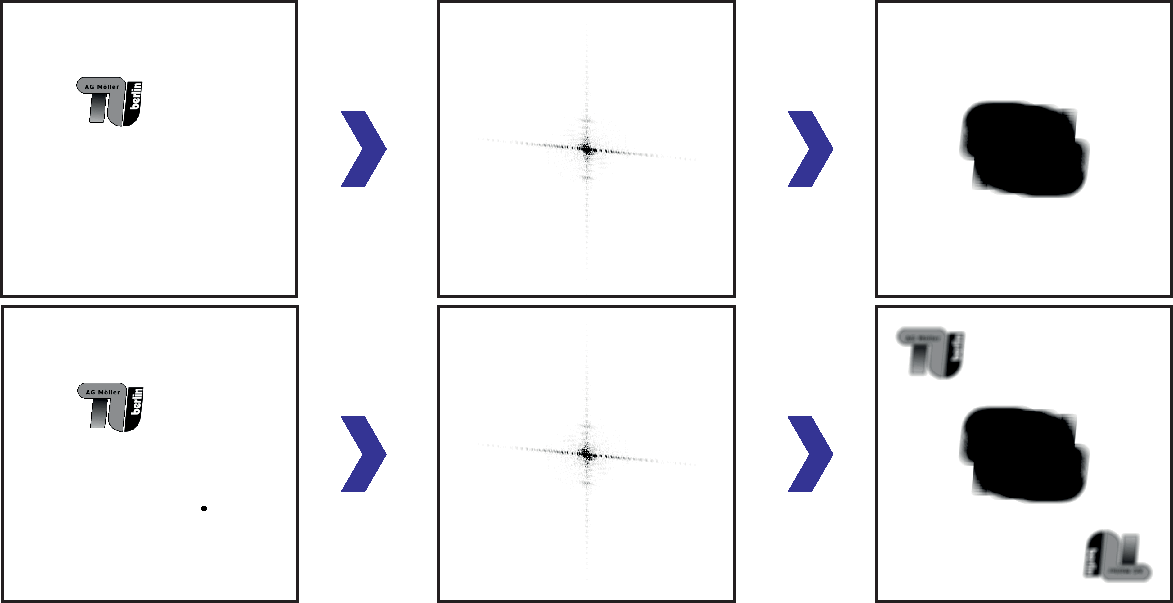
\includegraphics[width=0.75\textwidth]{images/fth.pdf}
	\caption[Prinzip Fouriertransformations-Holografie]{Prinzip der Fouriertransformations-Holografie: Wird von einem Objekt nur das Betragsquadrat der Fouriertransformierten aufgenommen, liefert die Rücktransformation die Autokorrelation des Objektes, aus der sich nur wenig über das ursprüngliche Objekt ableiten lässt (oben). Wird jedoch zusätzlich zu dem Objekt eine kleine Referenz genutzt, so liefert die Rücktransformation außerdem die Kreuzkorrelation aus Objekt und Referenz (unten).}
	\label{fig:fth}
\end{figure}

\subsection{Entfaltung}
Um bei ausgedehnten Referenzen eine bessere Approximation des Objektes zu erhalten, muss die Faltung zwischen Objekt und Referenz rückgängig gemacht werden. Nach \fref{eq:ft_faltung} entspricht die Faltung einer Multiplikation, die Inverse somit einer Division im Fourierraum. Jedoch verursachen vor allem zwei Effekte Probleme: i) Rauschen im aufgenommenen Bild, das bei der Division in Bereichen mit geringer Intensität der fouriertransformierten Referenz deutlich verstärkt werden würde und ii) Nullstellen der fouriertransformierten Referenz. 

Das Problem der Entfaltung tritt in verschiedenen Bereichen auf, unter anderem in der Bildverarbeitung.
Dort ist der Prozess der sogenannten \textit{Wiener-Entfaltung}, deren Prinzip für den eindimensionalen Fall in \fref{fig:wiener} dargestellt ist, etabliert. Hierbei wird der Wienerfilter $G$ für ein mit $H$ gefaltetes Signal $S$ mit additivem Rauschen (mit der spektralen Stärke $N$) definiert als
\begin{equation}
	G=\frac{H^* S}{\left|H\right|^2 S+N}\,.
\end{equation}
Für Rauschen, dass nicht mit dem Signal korreliert ist, minimiert eine Faltung mit $G$ die mittlere quadratische Abweichung zum rauschfreien, nicht gefalteten Original - es handelt sich somit im Sinne des mittleren quadratischen Fehlers um die ideale Entfaltung~\cite{castleman1996}. Ist das Rauschen jedoch mit dem Signal korreliert, wie dies z.B. bei Poisson-Rauschen (in Form des \textit{Schrotrauschen (engl. Shot Noise)} der größte Rauschbeitrag bei realen Streubildern) der Fall ist, so lässt sich eine heuristische Form des Wiener-Filters mit konstantem $N$ anwenden~\cite{he2004}. Dabei muss bei der Wahl von $N$ ein Kompromiss aus Rauschunterdrückung und Entfaltung gewählt werden.

\begin{figure}
	\centering
	\heximage{[width=.99\textwidth]{images/wiener.pdf}}
	\caption[Prinzip Enfaltung]{Prinzip der Holographie mit  Wiener Entfaltung: In der obersten Reihe sind Objekt und Referenz im Realraum (a) bzw. logarithmiert im Fourierraum (b) dargestellt. Wird das Betragsquadrat der Summe aus Objekt und Referenz im Fourierraum gebildet und in den Realraum rücktransformiert, so sind zentral die Autokorrelationen, außen die Kreuzkorrelationen zu erkennen (c). Wird die Kreuzkorrelation im logarithmierten Fourierraum betrachtet, so wird deutlich, dass bei niedrigen Raumfrequenzen das log. Objekt \textit{fast} die Differenz aus log. Kreuzkorrelation und log. Referenz ist, bei höheren Raumfrequenzen jedoch das Rauschen dominiert (d). Wenn im Fourierraum die Kreuzkorrelation durch die Referenz geteilt wird (\textit{direkte Entfaltung}), so wird bei Frequenzen, bei denen die Intensität der Referenz gering ist, das Rauschen deutlich verstärkt -- das Objekt ist nicht zu erkennen. Die \textit{Wiener-Entfaltung} verhindert dies, indem auch bei diesen Frequenzen eine "`Mindestintensität"' der Referenz in Höhe des geschätzten Rausch-zu-Signal-Verhältnisses verwendet wird (e und f). }
	\label{fig:wiener}
\end{figure} 

\section{Iterative Phasenrekonstruktion}
Wäre durch Aufnahme des Streubildes die vollständige komplexe Fouriertransformation der Austrittswelle (d.h. Amplitude und Phase) bekannt, so könnte die Austrittswelle einfach durch eine inverse Transformation gewonnen werden. Da die $N$ komplexen Datenpunkten im Realraum der Fouriertransformation durch $N$ Amplituden und $N$ Phasen, also $2N$ reelle Variablen dargestellt werden können, jedoch nur $N$ reelle Variablen (die Amplituden) gemessen werden können, ist das Problem unterbestimmt und nicht eindeutig lösbar. Kann jedoch das zu rekonstruierende Objekt im Realraum auf weniger als $N/2$ Bildpunkte beschränkt werden, so wird das Problem lösbar. Die räumliche Beschränkung im Realraum wird durch die Wahl eines sog. Supports umgesetzt, außerhalb dessen der Realraum als leer angenommen wird.  
Die Problemstellung ist nun im rauschfreien Fall eine Lösung der Gleichung $\rho(x)=\mathscr{F}^{-1}\tilde{\rho}(q)$ unter den Nebenbedingungen, dass i) $\rho$ auf den Support beschränkt ist und ii) die Amplituden von $\tilde{\rho}$ mit den gemessenen Fourieramplituden $A(q)$ übereinstimmen. Eine Lösung wird üblicherweise iterativ gefunden und stellt eine Wiederherstellung der Phase dar -- dieses Vorgehen wird deshalb als \textit{iterative Phasenrekonstruktion (IPR)} bezeichnet.
\subsection{Algorithmen}
Für die Lösung der Problemstellung existieren verschiedene Algorithmen, die im Folgenden vorgestellt werden. Eine detailliertere Beschreibung kann z.B. von Fienup oder Marchesini nachgelesen werden~\cite{marchesini2007,fienup1982}.
Der Prototyp der verwendeten Algorithmen, der \textit{Error-Reduction Algorithmus (ER)} basiert auf dem abwechselnden Erzwingen der Nebenbedingungen, d.h. von einem Startwert $\rho_0$ ausgehend wird zunächst $\tilde{\rho_0}$ bestimmt, die Amplitude im Fourierraum durch die gemessenen Amplituden $A$ ersetzt, in den Realraum transformiert und dort außerhalb des Supports gleich Null gesetzt. Dies wird iterativ wiederholt, wobei sich $\rho_n$ einer Lösung annähert, die beide Nebenbedingungen erfüllt~\cite{fienup1978}.

Eine Möglichkeit, sowohl den ER-Algorithmus wie auch die übrigen häufig verwendeten Algorithmen zu formulieren, sodass eine einheitliche Notation sowie graphische Darstellung möglich ist bietet die Notation mittels Projektionsoperatoren, die in \fref{fig:projektoren} skizziert sind:
Das Erzwingen der Nebenbedingung im Realraum kann als Projektion auf die Lösungsmenge $S$ der Nebenbedingung  (mit dem Komplement $\bar{S}$) durch den Projektor $P_s$ 

\begin{align}
	P_s\rho (x)=\begin{cases}
	\rho (x)  &\text{für } x\in S\\
	\mathbb{0}  &\text{für }x\notin S
	\end{cases} &   &   
	P_{\bar{s}}\rho (x)=\begin{cases}
	\mathbb{0} &\text{für } x\in S\\
	\rho (x)   &\text{für }x\notin S
	\end{cases}
\end{align}
aufgefasst werden. Der analoge Projektor für die Erfüllung der Nebenbedingung im Fourierraum, der im Fourierraum die Amplitude von $\tilde{\rho}$ durch die bekannte Amplitude $A(q)$ ersetzt und dabei die Phase $\Phi\left(\tilde{\rho}\left(q\right)\right)$ beibehält lautet
\begin{align}
	\tilde{P}_m \tilde{\rho}(q) & =A(q)e^{i\Phi(\tilde{\rho})} &   & P_m\rho(x)=\mathscr{F}^{-1}A(q)e^{i\Phi\left(\mathscr{F}\rho\left(x\right)\right)} \,. 
\end{align}

\begin{figure}
	\centering
	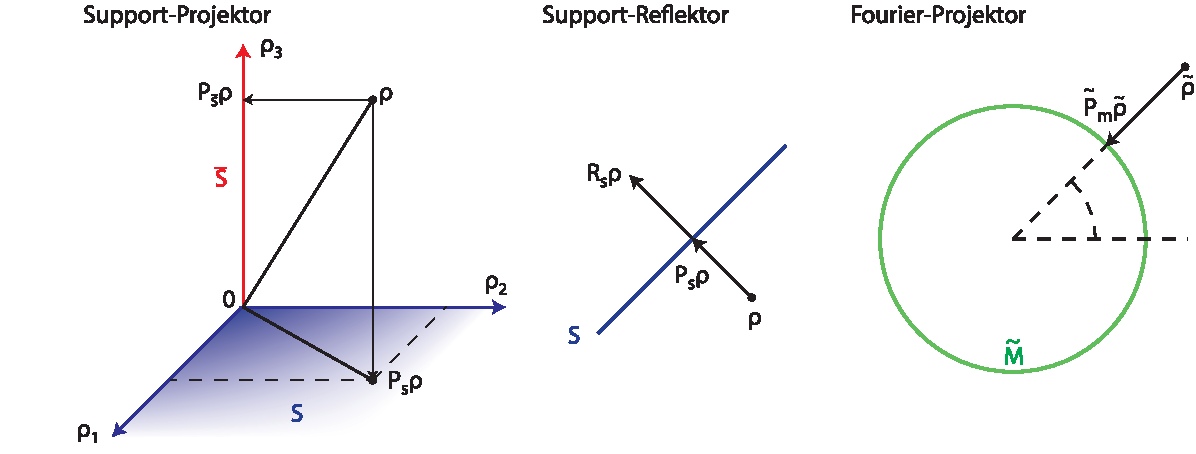
\includegraphics[width=1\textwidth]{images/projektor.pdf}
	\caption[Operatoren zur Beschreibung der Rekonstruktionsalgorithmen]{Zur Beschreibung der Rekonstruktionsalgorithmen verwendete Operatoren: Der Support-Projektor $P_S$ projiziert auf die durch den Support beschriebene Mannigfaltigkeit, $P_{\bar{S}}$ auf das Komplement. Ein Reflektor wendet die doppelte Schrittweite wie ein Projektor an und stellt somit eine Spiegelung an der Lösungsmenge der Nebenbedingung dar. Der Fourier-Projektor stellt in Fourierraum eine Projektion auf die kreisförmige Menge der bekannten Amplituden dar.}
	\label{fig:projektoren}
\end{figure}
Neben den Projektoren, die den Schritt $\rho \rightarrow P\rho = (\mathbb{1}+(P-\mathbb{1}))\rho$ ausführen, können auch sogenannte Reflektoren mit doppelter Schrittweite
\begin{equation}
	R_\nu= (\mathbb{1}+2(P_\nu-\mathbb{1}))=(2P_\nu-\mathbb{1})
\end{equation}
eingeführt werden.
In dieser Schreibweise können auch Weiterentwicklungen wie der \textit{Hybrid Input Output (HIO)} und  der \textit{Relaxed Averaged Alternating Reflections (RAAR)} Algorithmus dargestellt werden (siehe auch \fref{app:algos}). Ihre Prinzip ist in \fref{fig:recon} graphisch dargestellt. Die Algorithmen unterscheiden sich bezüglich ihres Konvergenzverhaltens und insbesondere bezüglich ihrer Anfälligkeit für Stagnation in lokalen Minima. 
Ein Rauschen im Fourierraum bewirkt, dass keine eindeutige exakte Lösung existieren muss, sondern nur ein globales Minimum aufgefunden werden kann. Dieses Problem tritt bei der Rekonstruktion experimentell aufgenommener Daten auf.
\begin{figure}
	\centering
	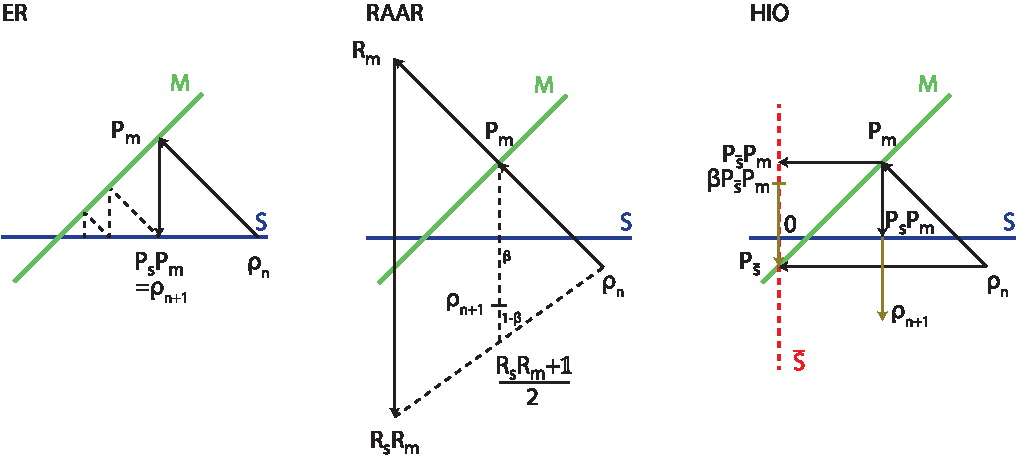
\includegraphics[width=1\textwidth]{images/algorithmen.pdf}
	\caption[Rekonstruktionsalgorithmen]{Darstellung der Algorithmen ER, RAAR und HIO: Bei ER findet eine abwechselnde Projektion auf die Lösungsmengen der Nebenbedingungen statt. Bei ER und HIO ist der einzelne Iterationsschritt komplexer und abhängig von einem Parameter $\beta$. Abbildung für ER und HIO nach~\cite{marchesini2007}. Für eine detailliertere Darstellung von RAAR und HIO siehe \fref{app:algos}}.
	\label{fig:recon}
\end{figure} 
\subsection{Support}
Üblicherweise ist der Bereich auf den das Objekt im Realraum beschränkt ist nicht bekannt, der für die iterativen Rekonstruktionsalgorithmen benötigte Support muss also zunächst bestimmt werden. Hierfür existieren verschiedene Möglichkeiten. Die triviale Methode besteht aus einer Festlegung aus zuvor bekannten Dimensionen des Experiments. Jedoch kann so nur in Ausnahmefällen der Support ausreichend eng gewählt werden, um die Bedingung, dass dieser weniger als $N/2$ Bildpunkte beinhalten muss, zu erfüllen.
Eine verbreitete Methode, bezeichnet als \textit{Shrink-Wrap} Algorithmus, ist durch eine Anpassung des Supports während der Rekonstruktion gekennzeichnet: Der zunächst geratene (für eine eindeutige Lösung des Problems  zu große) Support wird nach einer festgelegten Anzahl an Rekonstruktionsiterationen auf den Bereich beschränkt, in dem die rekonstruierte Intensität höher als ein festgelegter Schwellwert ist. Dieser aktualisierte Support wird für weitere Iterationen genutzt und erneut aktualisiert~\cite{marchesini2003}.

Die Nutzung der Holographie bietet eine weitere Methode der Bestimmung des Supports: Die aus der Holographie gewonnene Rekonstruktion des Objektes und eine Schätzung der Referenz lassen sich zu einem Support kombinieren. Hierfür wird nach Anwendung eines Median-Filters zur Rauschunterdrückung ein Schwellwert in Abhängigkeit von Mittelwert und der Standardabweichung der Rekonstruktion festgelegt. So kann nach morphologischem Öffnen und Schließen (zur Entfernung von Rauschen bzw. Löchern) die Kreuz- und Autokorrelation identifiziert werden\footnote{Details siehe \fref{app:param}.}. Der nötige Abstandsvektor dieser Supportteile ist der Abstandsvektor zwischen Auto- und Kreuzkorrelation (\fref{fig:support}).
In beiden Fällen ist darauf zu achten, dass der Support nicht zu klein gewählt wird, da es sonst keine Lösung unter dieser Nebenbedingung geben kann und somit die Algorithmen keine guten Rekonstruktion liefern, ein größerer als notwendiger Support bereitet hingegen (solange er weniger als $N/2$ Bildpunkte beinhaltet) kein Problem, es kann somit sinnvoll sein, den gewonnenen Support künstlich zu vergrößern~\cite{huang2010}.

\begin{figure}
	\centering
	\begin{subfigure}[b]{0.9\textwidth}
		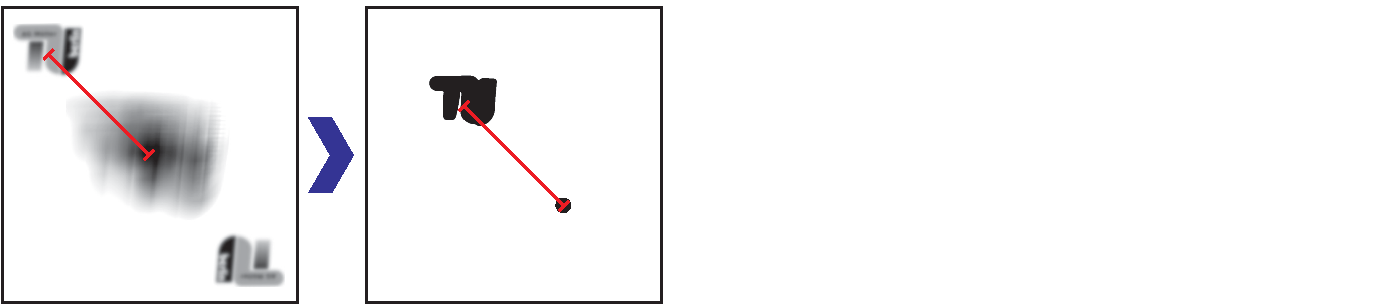
\includegraphics[width=\textwidth]{images/support_holo.pdf}
		\caption{Holographie}
	\end{subfigure}\\

	\begin{subfigure}[b]{0.9\textwidth}
		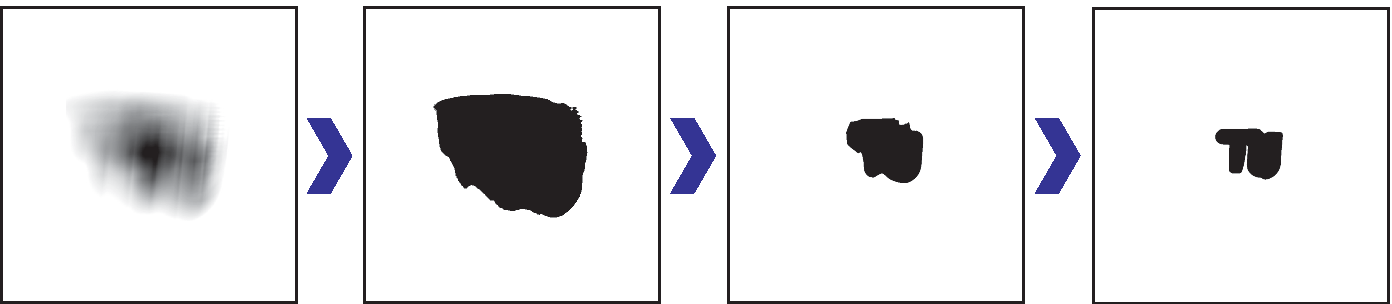
\includegraphics[width=\textwidth]{images/support_sw.pdf}
		\caption{Shrink-Wrap}	
	\end{subfigure}
	
	\caption[Supportgenerierung]{Erzeugung des Supports: Bei Verwendung von Holographie kann die Kreuzkorrelation aus Referenz und Objekt als Support genutzt werden. Zusätzlich muss im gleichen Abstand wie Kreuz- und Autokorrelation die Referenz dem Support hinzugefügt werden. Der Shrink-Wrap Algorithmus beginnt mit der Autokorrelation als initialem Support und passt diesen im Laufe der Rekonstruktion an.}
	\label{fig:support}
\end{figure} 

\subsection{Eindeutigkeit der Lösung}
Das Problem der IPR ist, dass die Algorithmen keine eindeutige Lösung liefern. Neben der Möglichkeit, dass die Algorithmen in einem lokalen Minimum stagnieren und dieses nicht verlassen, existiert eine weitere Quelle der Unsicherheit: Das sogenannte Zwillingsbild-Problem. Da nach \fref{eq:zwilling} das Bild $f(x,y)$ und das komplex konjugierte, punktgespiegelte "`Zwillingsbild"'  $f^*(-x,-y)$ den gleichen Betrag der Fouriertransformation besitzen, sind beides Lösungen des Problems.
\begin{equation}
	\label{eq:zwilling}
	\left|\mathscr{F}[f^*(-x,-y)]\right|=\left|\mathscr{F}[f(x,y)]^*\right|=\left|\mathscr{F}[f(x,y)]\right|
\end{equation}
Dies führt dazu, dass bei einem punktsymmetrischen Support (oder einem Support, der so groß ist, dass Bild und Zwillingsbild in ihn hineinpassen) in einigen Regionen das Bild, in anderen das Zwillingsbild rekonstruiert wird. Beide Probleme, Stagnation im Minimum und Zwillingsproblem, sind abhängig von der Wahl des Startpunktes der Rekonstruktion, bei zufälliger Wahl der Fourierphase ist die Rekonstruktion somit nicht deterministisch.

Der Shrink-Wrap-Algorithmus zur Supportgewinnung kann das Zwillingsproblem in manchen Fällen umgehen, indem bei einer Dominanz von Bild oder Zwillingsbild in einem der Randbereiche des aktuellen Supports das jeweils andere bei der nächsten Anpassung des Supports unterdrückt wird und so ein nicht-punktsymmetrischer Support gefunden werden kann.
Die Supportgewinnung mittels Holographie löst dieses Problem vollständig. Je nach Wahl der für den Support verwendeten Kreuzkorrelation und davon abhängiger Platzierung der Referenz im Support wird Bild oder Zwillingsbild rekonstruiert, da Objekt und Referenz zusammen nicht punktsymmetrisch sind.

Für die IPR wird häufig mehrfach mit verschiedenen, zufälligen Fourierphasen gestartet und ein Mittelwert aus den Rekonstruktionen gebildet (hierbei müssen die einzelnen Rekonstruktionsergebnisse hinsichtlich Translation und Punktspiegelung angepasst werden). Die Methode der Kombination aus FTH zur Supportgewinnung und anschließender IPR beginnt jedoch mit einem definierten Start (der Kreuzkorrelation) und wird nur einmalig durchgeführt. Das Ergebnis der Rekonstruktion jedes einzelnen Streubildes ist somit eindeutig und es handelt sich um ein deterministisches Verfahren.

\section{Vergleich in 2D}	
Es können nun die drei unterschiedliche Arten der Rekonstruktion verglichen werden:
\begin{itemize}
	\item FTH mit Entfaltung
	\item IPR mit Shrink-Wrap Support
	\item IPR mit FTH Support
\end{itemize}
Die Rekonstruktionsansätze werden bezüglich Ihrer Empfindlichkeit gegenüber Rauschen, gegenüber den durch zentrale Maskierung des Streubildes entstehenden Hochpass und gegenüber einem Fehler in der Abschätzung der Referenz untersucht. Dies geschieht zunächst mit rein synthetischen 2D Bildern als Ersatz für Austrittswellen, um die Funktion der drei Ansätze und ihre Limitationen zu überprüfen.

Als Algorithmus der IPR wird bei diesem Vergleich ein Wechsel aus HIO ($\beta=0.9$) und ER verwendet, die genauen Parameter und Abläufe sind in \fref{app:param} angegeben. Diese Kombination wird aufgrund ihrer großen Verbreitung in der Literatur stellvertretend für die IPR betrachtet\footnote{Die Verwendung von RAAR liefert keine signifikant abweichende Aussagen und wird daher im folgenden nicht dargestellt.}. 

Bei idealen Bedingungen, d.h. ohne Rauschen, ohne zentrale Maskierung und mit präzise bekannter Referenz liefern, wie in \fref{fig:recon2d-perfect} zu erkennen, alle Ansätze ein optisch vom Ausgangsbild nicht zu unterscheidendes Ergebnis.

\begin{figure}
	\centering
	\reconimage{[width=.48\textwidth]{images/recon2d-perfect.png}}
	\caption[2D Rekonstruktion: Ideal]{Rekonstruktion mit Zentralstrahl ohne Rauschen: Oben links das theoretische Optimum, in diesem Falle das Eingangsbild, bei späteren Bildern mit maskierter Mitte das hochpassgefilterte Eingangsbild. Oben rechts die durch IPR mit Shrink-Wrap, unten links die durch Entfaltung (mit dem Parameter $N=1$) aus der FTH gewonnene Rekonstruktion. Unten rechts die Rekonstruktion mittels IPR mit FTH als Start und Support. Alle Rekonstruktionen liefern optisch perfekte Ergebnisse. }
	\label{fig:recon2d-perfect}
\end{figure}

\subsection{Einfluss der Zentralmaske}
Bei der Aufnahme von Streubildern in Experimenten wird aufgrund der großen Intensität des ungestreuten Strahles zur Vermeidung der Beschädigung des Detektors der zentrale Anteil des Strahles blockiert~\cite{schultz2013chapter7}. Dies wirkt in der Fraunhofer-Fernfeldnäherung wie ein Hochpass. Der Einfluss dieses Hochpasses zeigt sich in \fref{fig:recon2d-mask}, in der die Ergebnisse der Rekonstruktion bei geringer und größerer Maskierung der zentralen Anteile des Streubildes der verschiedenen Ansätze dargestellt sind. An dieser Stelle sei darauf hingewiesen, dass durch die Festlegung eines räumlich beschränkten Supports mehr Informationen rekonstruiert werden könnten, als durch einen Hochpass nahe gelegt: Wie in \fref{fig:missing} illustriert sind durch die Festlegung eines Supports im Realraum auch die vom Hochpass betroffenen Frequenzanteile nicht mehr vollkommen frei wählbar. Für eine korrekte Betrachtung der tatsächlich fehlenden Informationen muss das Eingangsbild in eine Basis aus sowohl im Real- wie auch im Fourierraum räumlich beschränkte Funktionen zerlegt werden. Nur die Komponenten, die sowohl im Fourierraum vollständig im maskierten Bereich liegen, wie auch im Realraum vollständig im Support liegen, können nicht wieder rekonstruiert werden~\cite{thibault2006,ulmer2015}. Jedoch ist die optische Beurteilbarkeit so rekonstruierter Bilder eingeschränkt. Aus diesem Grund sind die dargestellten Bilder hochpassgefiltert, um einen gewohnten Bildeindruck zu vermitteln.
\begin{figure}
	\centering
	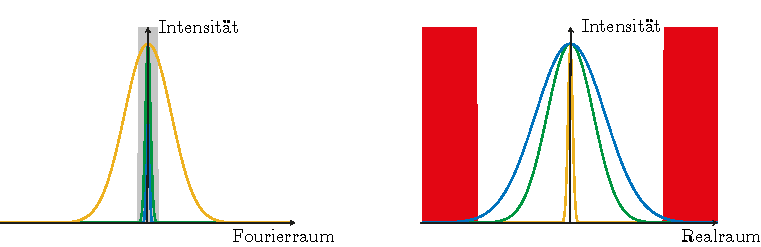
\includegraphics[width=.9\textwidth]{images/missing.pdf}
	\caption[Fehlende Bildinformationen]{Illustration zu den fehlenden Bildinformationen: Auch wenn im Fourierraum ein Teil des Bildes nicht bekannt ist (grau dargestellt), so können dort aufgrund der Supportbeschränkung im Realraum (rot dargestellt) nicht beliebige Intensitäten liegen. In diesem Beispiel mit drei reinen Gauß-Funktionen könnte sowohl die blau wie auch die grün dargestellte Funktion im unbekannten Bereich liegen, die Realraumbeschränkung verbietet jedoch die blaue Funktion. Somit bewirkt das Einführen eines Supports eine Einschränkung der unbekannten Informationen, die über einen reinen Hochpass hinaus geht.}
	\label{fig:missing}
\end{figure}
Sowohl die Wiener-Entfaltung als auch die IPR mit Support aus der Holographie erzeugen optisch ideale Rekonstruktionen, die Erzeugung des Supports mittels Shrink-Wrap ist stärker beeinflusst, liefert aber ebenfalls gute Ergebnisse in Abwesenheit von Rauschen.
\begin{figure}
	\begin{subfigure}[b]{0.48\textwidth}
		\reconimage{[width=\textwidth]{images/recon2d-mask16.png}}
		\caption{kleine Maske}
	\end{subfigure}
	\hspace*{\fill}
	\begin{subfigure}[b]{0.48\textwidth}
		\reconimage{[width=\textwidth]{images/recon2d-mask64.png}}
		\caption{große Maske}	
	\end{subfigure}
	\caption[2D Rekonstruktion: Beamstop]{Einfluss einer zentralen Maskierung des Streubildes mit Radius 16 Pixel bzw. 64 Pixel von 2048 Pixeln auf die Rekonstruktionen (gleiche Anordnung wie in \fref{fig:recon2d-perfect}). Die Entfaltung ($N=1$) erweist sich als am unempfindlichsten, die IPR als am empfindlichsten.}
	\label{fig:recon2d-mask}
\end{figure}

\subsection{Einfluss des Rauschens}
Zur Beurteilung des Einflusses von Rauschen auf die Rekonstruktionen werden die Fourieramplituden mit verschiedenen Auflösungen diskretisiert und ein Poisson-Rauschen angewendet (\fref{fig:recon2d-noise}). Dadurch wird das natürliche Schrotrauschen bei idealer Belichtung simuliert. Hier zeigt sich eine Unempfindlichkeit der Wiener-Entfaltung gegenüber Rauschen -- durch den Rauschterm in der Entfaltung kann der störende Einfluss minimiert und gleichzeitig eine ausreichende Entfaltung bewirkt werden. Insbesondere die IPR mit Shrink-Wrap Support leidet unter Rauschen, da kein geeigneter Support gefunden werden kann. Durch die Erzeugung des Supports mittels Holographie kann dieses Problem umgangen werden.
\begin{figure}
	\begin{subfigure}[b]{0.45\textwidth}
		\reconimage{[width=\textwidth]{images/recon2d-mask16bit16.png}}
		\caption{wenig Rauschen}
	\end{subfigure}
	\hspace*{\fill}
	\begin{subfigure}[b]{0.45\textwidth}
		\reconimage{[width=\textwidth]{images/recon2d-mask16bit14.png}}
		\caption{viel Rauschen}	
	\end{subfigure}
	\caption[2D Rekonstruktion: Rauschen]{Einfluss des Rauschen: Das gering maskierte Streubild wurde mit 16\,Bit bzw. 14\,Bit diskretisiert und Poisson-Rauschen hinzugefügt. Die Entfaltung ($N=\num{1e3} \text{ bzw. }\num{3e3}$) erweist sich deutlich als am unempfindlichsten, die IPR als am empfindlichsten.}
	\label{fig:recon2d-noise}
\end{figure}
\subsection{Einfluss der Referenzabschätzung}
Sowohl für die Entfaltung wie auch für die Festlegung des Supports für die IPR muss die Referenz abgeschätzt werden. Der Einfluss der Güte dieser Abschätzung lässt sich in \fref{fig:recon2d-ref} betrachten. Schon eine Abweichung des Radius von 5~\% von der wahren Größe bewirkt ein Scheitern der Entfaltung. Die iterativen Algorithmen sind hingegen unempfindlich gegenüber diesem Einfluss.

Zusammenfassend lässt sich aus der zweidimensionalen Untersuchung die Anfälligkeit der IPR bezüglich Rauschen und fehlenden Bildinformationen sowie die Anfälligkeit der Wiener-Entfaltung bezüglich einer nicht perfekt bekannten Referenz bei relativer Unempfindlichkeit gegenüber den zuvor genannten Effekten hervorheben. Die Kombination aus Entfaltung zur Gewinnung des Supports und Verfeinerung mittels iterativer Rekonstruktion scheint die Vorteile beider Verfahren zu kombinieren.
\begin{figure}
	\begin{subfigure}[b]{0.45\textwidth}
		\reconimage{[width=\textwidth]{images/recon2d-mask16bit16error01.png}}
		\caption{1~\% Abweichung des Radius}
	\end{subfigure}
	\hspace*{\fill}
	\begin{subfigure}[b]{0.45\textwidth}
		\reconimage{[width=\textwidth]{images/recon2d-mask16bit16error05.png}}
		\caption{5~\% Abweichung des Radius}	
	\end{subfigure}
	\caption[2D Rekonstruktion: Referenz]{Einfluss von ungenauer Referenzabschätzung: Das gering verrauschte und maskierte Streubild wird mit einem anderen Radius der kreisförmigen Referenz rekonstruiert. Dies hat nur einen Einfluss auf die Entfaltung ($N=\num{2e3} \text{ bzw. }\num{2e4}$).}
	\label{fig:recon2d-ref}
\end{figure}
 \clearpage
\section{Rekonstruktion einer 3D Austrittswelle}
Die für zweidimensionale Bilder getesteten Ansätze können nun zur Rekonstruktion der Austrittswelle hinter einem dreidimensionalen Objekt eingesetzt werden. In \fref{fig:recon3d} wird die Austrittswelle analog zu den 2D-Bildern betrachtet.
	
Die Entfaltung wurde mit einer simulierten Austrittswelle der Referenz durchgeführt. Obwohl hierfür von einer vollständig bekannten Referenz ausgegangen wird, leidet die Rekonstruktion deutlich unter der komplexen Struktur und der Diskretisierung der Referenz. Die IPR leidet hingegen sichtbar unter Zwillingsbildern. Dieses Problem kann durch die Kombination von IPR und Holographie umgangen werden. Das Ergebnis dieser Kombination unterscheidet sich optisch kaum von der Austrittswelle direkt hinter dem Objekt.

\begin{figure}
	\centering
	\quadimage{[width=.75\textwidth]{images/recon3d-v2.png}}
	\caption[Rekonstruktion einer Austrittswelle]{Die Rekonstruktion einer komplexen Austrittswelle: Dargestellt ist jeweils das Ergebnis der Rekonstruktion der Austrittswelle aus \fref{fig:komplex} (mit der von dort bekannten Farbskala) normiert auf das optimale Ergebnis (a). Die Rekonstruktion mittels IPR mit Shrink-Wrap (b) leidet unter Zwillingsbildern, die Kombination aus IPR und Holographie (d) ist optisch gut und der reinen Entfaltung (c) überlegen.}
	\label{fig:recon3d}
\end{figure}

Durch eine Anwendung einer Propagation lässt sich die Fokusebene sowohl der idealen wie auch der rekonstruierten Austrittswelle verschieben~\cite{ulmer2015}. Wird hierbei als Schärfekriterium die Varianz genutzt und diese maximiert, so wird eine Ebene innerhalb des Objektes "`fokussiert"'. Zu beachten ist, dass hierbei nicht das Wellenfeld an dieser Position berechnet wird, sondern ein in der Realität nicht vorliegendes Bild erzeugt wird, dass jedoch für die optische Beurteilung aufgrund der erhöhten Schärfe besser geeignet ist.  Bei dieser in \fref{fig:recon_focus} dargestellten Fokussierung ist die rekonstruierte Austrittswelle optisch kaum vom idealen Ergebnis zu unterscheiden.

\begin{figure}
	\centering
	\dualimage{[width=.85\textwidth]{images/recon3d-v2_focus.png}}
	\caption[Propagation der Austrittswelle]{Durch Anwendung einer Propagation um \SI{-50}{nm}  lässt die Schärfe der idealen Austrittswelle (a) bzw. einer Propagation um \SI{30}{nm} der durch Kombination von Entfaltung und iterativer Rekonstruktion gewonnene Welle (b) maximieren. Sie unterscheiden sich in diesem Falle optisch kaum.}
	\label{fig:recon_focus}
\end{figure}

Somit ist auch für die Rekonstruktion einer komplexen Austrittswelle die Kombination aus Holographie und IPR gut geeignet.